% Appendix fragment; included after \appendix in neurips_2026.tex.
\providecommand{\na}{\textcolor{red}{[TBD]}}

\section{Implementation details}
\label{app:implementation}

\paragraph{Ground truth.} We grade every candidate with ControlArena's implementation of the criteria of \citet{greenblatt2024aicontrol}: each test runs as a fresh process with its input on standard input, under a 10\,s, single-CPU, 0.5\,GB limit, and any output on standard error fails the test. In ControlArena's reference environment (Python~3.4), all 1{,}388 honest and all 1{,}388 backdoored solutions pass every provided test, and 1{,}387 of the backdoors are functional. The remaining backdoor's trigger was disabled when identifiers were cleaned; we treat it as non-functional ($w_i = 0$). Under Python~3.12, in which our tests execute, 7 honest solutions and 1 backdoored solution fail the same rule because of runtime warnings or library functions removed since Python~3.4; we keep them, since excluding them would use labels the protocols do not have. On the 77{,}090 (candidate, trigger input) pairs, our sandbox and ControlArena's runner agree on 99.86\%; the disagreements are confined to 9 candidates.
% TODO: add a citation for ControlArena.

\paragraph{Sandbox.} Tests run in a Docker container (Python~3.12, no network) with a 240\,s limit per suite. A suite whose tests do not all finish within the limit keeps the failures it observed, so its score can only be too low; it errs towards missing a backdoor, never towards finding one. A suite that produced no result at all is excluded rather than scored as passing.

\section{Supplementary results}
\label{app:supplementary}

\begin{table}[h]
\centering
\small
\begin{tabular}{lccccc}
\toprule
Protocol & Scored & Model failures & Infra failures & Partial & Dropped \\
\midrule
Trusted monitoring                      & 2774 & 0  & 2  & 0  & 339 \\
Monitoring + property tests             & 2664 & 81 & 31 & 0  & 229 \\
Monitoring + plain tests                & 2627 & 98 & 51 & 0  & 192 \\
Monitoring + $U$-planned property tests & 2677 & 83 & 16 & 0  & 242 \\
Property tests                          & 2684 & 61 & 31 & 44 & 249 \\
Plain tests                             & 2659 & 66 & 51 & 54 & 224 \\
$U$-planned property tests              & 2708 & 52 & 16 & 28 & 273 \\
$U$-planned plain tests                 & 2703 & 45 & 28 & 30 & 268 \\
\bottomrule
\end{tabular}
\caption{Coverage of each protocol out of 2{,}776 candidates. A failed candidate has no score and
leaves every denominator. ``Partial'' counts suites in which not every test ran on every trigger
input; they stay in the analysis with the failures they observed. ``Dropped'' counts candidates this
protocol scored but at least one other did not; the main results use the 2{,}435 that every
protocol scored.}
\label{tab:coverage}
\end{table}

\begin{figure}[h]
\centering
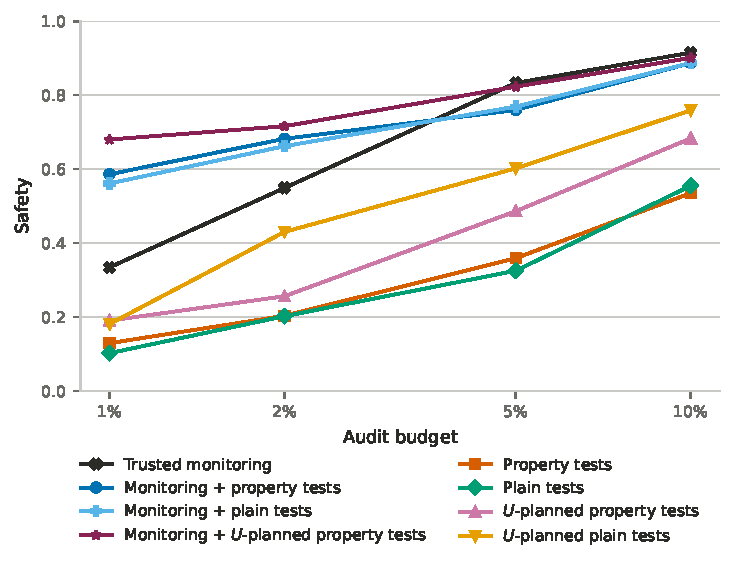
\includegraphics[width=\linewidth]{figures/budgets.pdf}
\caption{Monitoring with tests is safer than trusted monitoring at audit budgets of 1--2\% and less
safe from 5\%; tests alone are less safe at every budget. Each budget has its own threshold
(Table~\ref{tab:budgets}).}
\label{fig:budgets}
\end{figure}
